\documentclass[11pt,a4paper]{article}
\usepackage[utf8]{inputenc}
\usepackage[T1]{fontenc}

\usepackage[margin=2.4cm]{geometry}
\usepackage{amsmath,amssymb}
\usepackage{siunitx}
\usepackage{booktabs,array}
\usepackage{graphicx}
\usepackage{float}
\usepackage[font=small,labelfont=bf]{caption}
\usepackage{subcaption}
\usepackage{fancyhdr}
\usepackage{enumitem}
\usepackage[hidelinks]{hyperref}

\usepackage{tikz}

\sisetup{separate-uncertainty=true,detect-all}
\setlength{\parindent}{0pt}
\setlength{\parskip}{6pt}
\renewcommand{\arraystretch}{1.15}
\setlength{\headheight}{14pt}
\pagestyle{fancy}
\fancyhf{}
\lhead{UP 201 -- Experiment 7}
\rhead{Bragg's Law and Absorption of X-rays}
\cfoot{\thepage}
\renewcommand{\headrulewidth}{0.4pt}

\newcommand{\Ka}{K$_\alpha$}
\newcommand{\Kb}{K$_\beta$}
\newcommand{\dd}{\mathrm{d}}
\newcommand{\eu}{\mathrm{e}}

\begin{document}

%================== TITLE ==================
\begin{titlepage}
\centering
\vspace*{1.5cm}
{\large UP 201 \,--\, Physics Laboratory}\\[0.4cm]
{\Large Experiment 5}\\[1.2cm]
{\Huge\bfseries Bragg's Law and Absorption of X-rays}\\[0.6cm]
\rule{0.8\textwidth}{0.6pt}\\[0.6cm]
{\large Cu-anode X-ray unit \,$\bullet$\, LiF and KBr single crystals \,$\bullet$\, GM counter \,$\bullet$\, Al absorbers}\\[3cm]
\begin{tabular}{rl}
\textbf{Parth}\\[0.5cm]
\textbf{26788}\\[0.5cm]
\textbf{28 Sept 2026}\\[0.5cm]
\end{tabular}
\vfill
\end{titlepage}

%================== INDEX ==================
\pagenumbering{roman}
\tableofcontents
\clearpage
\listoffigures
\listoftables
\clearpage
\pagenumbering{arabic}

%================== 1. AIM ==================
\section{Aim}
\begin{enumerate}[label=\arabic*.]
\item To set up the X-ray unit, record the X-ray spectrum of the Cu anode with a LiF crystal, study the continuous and characteristic X-rays and determine the wavelength and energy of the characteristic \Ka\ and \Kb\ lines (with uncertainties).
\item To determine the inter-planar spacing of a KBr crystal using the characteristic lines.
\item To determine the attenuation of X-rays in aluminium and the mass attenuation coefficient $\mu/\rho$ as a function of wavelength.
\end{enumerate}

\section{Apparatus}
PHYWE X-ray unit (35\,kV maximum) with Cu-anode Coolidge tube, goniometer with $1{:}2$ crystal--detector coupling, 1\,mm and 5\,mm apertures, LiF and KBr single crystals, Geiger--M\"uller (GM) counter tube, aluminium absorbers (0.02, 0.04, 0.06, 0.08 and 0.10\,mm), computer with \emph{measure} software.

%================== 3. PRINCIPLE ==================
\section{Principle and Theory}

\subsection{Production of X-rays and the spectrum of an X-ray tube}
Electrons emitted thermionically from the heated cathode are accelerated through the anode voltage $U_A$ and strike the Cu anode with kinetic energy $eU_A$. Two kinds of radiation are produced.

\paragraph{Continuous spectrum (Bremsstrahlung).} An electron decelerated in the Coulomb field of the anode nuclei radiates part of its energy as a photon; since the energy loss can take any value, the spectrum is continuous. The most energetic photon is emitted when the electron gives \emph{all} its kinetic energy to a single photon (Duane--Hunt law):
\begin{equation}
eU_A = h\nu_{\max} = \frac{hc}{\lambda_{\min}}
\quad\Longrightarrow\quad
\lambda_{\min}=\frac{hc}{eU_A}=\frac{1.2398\ \si{\nano\metre\kilo\volt}}{U_A}.
\label{eq:duane}
\end{equation}
For $U_A=\SI{35}{\kilo\volt}$ this gives $\lambda_{\min}=35.42\ \si{\pico\metre}$, \emph{independent of the anode material}.

\paragraph{Characteristic spectrum.} If an incident electron ejects a K-shell electron of a Cu atom, the vacancy is filled by an electron from a higher shell and the energy difference is emitted as a photon of fixed energy. For $L\to K$ and $M\to K$ transitions
\begin{equation}
E_{K_\alpha}=|E_K|-|E_L|,\qquad E_{K_\beta}=|E_K|-|E_M| ,
\end{equation}
which depend only on the atomic levels of Cu, not on $U_A$ (provided $eU_A$ exceeds the K-binding energy, $\approx\SI{8.98}{\kilo\electronvolt}$). They appear as sharp lines superimposed on the continuum. Literature values for Cu are $E_{K_\alpha}\approx\SI{8.048}{\kilo\electronvolt}$ ($\lambda=\SI{154.2}{\pico\metre}$) and $E_{K_\beta}\approx\SI{8.905}{\kilo\electronvolt}$ ($\lambda=\SI{139.2}{\pico\metre}$).

\subsection{Crystal structure and Bragg's law}
\paragraph{Derivation of Bragg's law.}
Consider a monochromatic beam of wavelength $\lambda$ incident at glancing angle $\theta$ on a family of parallel lattice planes of spacing $d$ (Fig.~\ref{fig:bragg}). Each plane reflects a small fraction of the beam specularly. Two rays reflected from adjacent planes travel different distances: the lower ray covers the extra path $AB+BC$, where $AB=BC=d\sin\theta$. The path difference is therefore
\begin{equation}
\Delta = AB+BC = 2d\sin\theta .
\end{equation}
The reflected rays reinforce each other (constructive interference) only if $\Delta$ is an integral number of wavelengths:
\begin{equation}
\boxed{\,2d\sin\theta = n\lambda\,},\qquad n=1,2,3,\dots
\label{eq:bragg}
\end{equation}
Since the sum over many planes cancels the intensity at all other angles, sharp peaks appear at the Bragg angles $\theta_n=\arcsin\!\big(n\lambda/2d\big)$. A polychromatic beam is thus \emph{dispersed}: each wavelength satisfies Eq.~\eqref{eq:bragg} at a different angle, which lets the crystal act as a spectrometer. Because $\sin\theta\le1$, only wavelengths with $\lambda\le 2d/n$ are diffracted.

\begin{figure}[H]
\centering
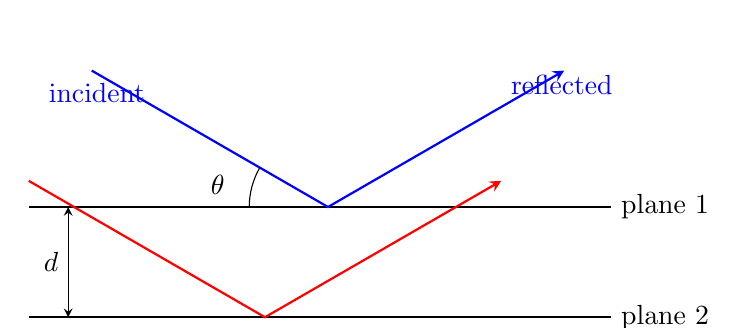
\begin{tikzpicture}[>=stealth,scale=1.0]
\foreach \y in {0,-1.4} \draw[thick] (-0.8,\y) -- (6.6,\y);
\node[right] at (6.6,0) {plane 1};\node[right] at (6.6,-1.4) {plane 2};
\draw[->,thick,blue] (0,1.732) -- (3,0) -- (6,1.732);
\draw[->,thick,red] (-0.8,0.332) -- (2.2,-1.4) -- (5.2,0.332);
\node[blue,above left] at (0.8,1.2) {incident};\node[blue,above right] at (5.2,1.3) {reflected};
\draw (2,0) arc (180:150:1);\node at (1.6,0.28) {$\theta$};
\draw[<->] (-0.3,0) -- (-0.3,-1.4);\node[left] at (-0.3,-0.7) {$d$};
\end{tikzpicture}
\caption{Geometry for Bragg's law (schematic, drawn as text: incident and reflected rays at glancing angle $\theta$ from planes separated by $d$; extra path $=2d\sin\theta$).}
\label{fig:bragg}
\end{figure}

\paragraph{Lattice spacing in a cubic crystal.} For a cubic crystal of lattice constant $a$, the planes with Miller indices $(hkl)$ have spacing
\begin{equation}
d_{hkl}=\frac{a}{\sqrt{h^2+k^2+l^2}} .
\end{equation}
LiF, KBr and NaCl all have the rock-salt structure (two interpenetrating face-centred-cubic lattices of cations and anions). The strongest reflection is from the $(200)$ planes, $d_{200}=a/2$; higher orders $n=2,3,4$ of $(200)$ are the $(400),(600),(800)$ reflections. For LiF, $a\simeq\SI{402.7}{\pico\metre}$ so $d=\SI{201.4}{\pico\metre}$ (value used in the experiment).

\paragraph{$1{:}2$ coupling.} In the goniometer the crystal is rotated through $\theta$ while the counter is rotated through $2\theta$, so the counter always sits at the direction of the reflected beam (angle between incident and reflected beams $=2\theta$).

\subsection{Geiger--M\"uller counter and dead-time correction}
Each ionising photon produces a voltage pulse. After a pulse the GM tube is insensitive for a time $\tau$ (the \emph{dead time}). Let $N$ be the true rate of photons arriving and $N_0$ the measured rate. In one second the counter is dead for a total time $N_0\tau$ (each of the $N_0$ recorded pulses is followed by a dead interval $\tau$), so it is live for $1-N_0\tau$ seconds. Photons arriving during this live time are all counted:
\begin{equation}
N\,(1-N_0\tau)=N_0
\quad\Longrightarrow\quad
\boxed{\,N=\frac{N_0}{1-\tau N_0}\,}
\label{eq:dead}
\end{equation}
(inversely, $N_0=N/(1+\tau N)$). The correction is negligible for $\tau N_0\ll1$ and diverges as $N_0\to1/\tau$. If the rate $N_0$ has statistical error $\sigma_{N_0}=\sqrt{N_0/t_g}$ for gate time $t_g$, then
\begin{equation}
\sigma_N=\frac{\partial N}{\partial N_0}\,\sigma_{N_0}=\frac{\sigma_{N_0}}{(1-\tau N_0)^2}.
\label{eq:sigmaN}
\end{equation}

\subsection{Absorption of X-rays}
\paragraph{Beer--Lambert law.} In a thin layer $\dd x$ of an absorber the fractional loss of intensity is proportional to the thickness: $\dd I=-\mu I\,\dd x$, where $\mu$ is the linear attenuation coefficient. Integrating from $x=0$ ($I=I_0$) to $x=d$:
\begin{equation}
\int_{I_0}^{I}\frac{\dd I}{I}=-\mu\int_0^d \dd x\ \Longrightarrow\ I=I_0\,\eu^{-\mu d}
\quad\Longleftrightarrow\quad
\ln I=\ln I_0-\mu d .
\label{eq:beer}
\end{equation}
A plot of $\ln I$ against $d$ at fixed wavelength is a straight line of slope $-\mu$. Since absorption is proportional to the mass traversed, the density-independent \emph{mass attenuation coefficient} $\mu/\rho$ (cm$^2$\,g$^{-1}$) is used; $\rho_{\rm Al}=\SI{2.70}{\gram\per\cubic\centi\metre}$.

\paragraph{Interaction processes.}
\begin{itemize}[nosep]
\item \emph{Photoelectric effect (PE):} the photon is absorbed by a bound electron, which is ejected with $E_{kin}=h\nu-E_{\rm binding}$.
\item \emph{Compton scattering (CS):} the photon scatters from a (quasi-free) electron and loses energy. Conservation of energy and momentum gives $\lambda'-\lambda=\dfrac{h}{m_0c}\,(1-\cos\varphi)$.
\item \emph{Pair production:} a photon creates an $e^-e^+$ pair in the field of a nucleus; energy conservation requires $h\nu\ge 2m_0c^2=\SI{1.022}{\mega\electronvolt}$.
\end{itemize}
In the keV range pair production is energetically forbidden, so
\begin{equation}
\mu=\mu_{PE}+\mu_{CS}.
\end{equation}
For low-energy photons and a light absorber such as Al, PE dominates over CS. Between absorption edges the mass attenuation coefficient follows the empirical relation
\begin{equation}
\frac{\mu}{\rho}=C\,Z^{3}\lambda^{3},
\label{eq:lambda3}
\end{equation}
($Z$ = atomic number, $C$ = constant); the $\lambda^3$ ($\propto E^{-3}$) dependence reflects the photoelectric cross-section. A plot of $\ln(\mu/\rho)$ versus $\ln\lambda$ should therefore be a straight line of slope $\approx3$.

\subsection{Least-squares fitting and error propagation}
For $y=a+bx$ with weights $w_i=1/\sigma_i^2$:
\begin{equation}
b=\frac{S\,S_{xy}-S_xS_y}{S\,S_{xx}-S_x^2},\quad
a=\frac{S_y-bS_x}{S},\quad
\sigma_b=\sqrt{\frac{S}{S\,S_{xx}-S_x^2}},
\end{equation}
with $S=\sum w_i$, $S_x=\sum w_ix_i$, $S_y=\sum w_iy_i$, $S_{xx}=\sum w_ix_i^2$, $S_{xy}=\sum w_ix_iy_i$. When the reduced $\chi^2_\nu>1$, $\sigma_b$ is multiplied by $\sqrt{\chi^2_\nu}$. Other propagation formulae used (all derived from $\sigma_f^2=\sum(\partial f/\partial x_i)^2\sigma_i^2$):
\begin{align}
\lambda&=\frac{2d\sin\theta}{n} &\Rightarrow\quad \sigma_\lambda&=\lambda\cot\theta\,\sigma_\theta\ \ (\sigma_\theta\text{ in rad}),\\
E&=\frac{hc}{\lambda}=\frac{1239.84\ \si{\electronvolt\nano\metre}}{\lambda} &\Rightarrow\quad \frac{\sigma_E}{E}&=\frac{\sigma_\lambda}{\lambda},\\
\frac{\mu}{\rho}&=\frac{\mu}{\rho} &\Rightarrow\quad \sigma_{\mu/\rho}&=\frac{\sigma_\mu}{\rho}.
\end{align}

%================== 4. PROCEDURE ==================
\section{Brief Procedure}
\begin{enumerate}[nosep]
\item The 1\,mm aperture was mounted on the X-ray outlet, the LiF crystal placed in the goniometer holder and the goniometer calibrated (under the supervision of the instructor).
\item In the \emph{measure} software: $1{:}2$ coupling mode, gate time 2\,s, angular step $0.1^\circ$, $U_A=\SI{35}{\kilo\volt}$, $I_A=\SI{1}{\milli\ampere}$; the spectrum was scanned from $6^\circ$ to $55^\circ$ (LiF) and the stored data corrected for dead time using Eq.~\eqref{eq:dead}.
\item The LiF crystal was replaced by KBr and scanned from $6^\circ$ to $75^\circ$.
\item For absorption the aperture was changed to 5\,mm and the LiF crystal was used. With each Al absorber (0, 0.02, 0.04, 0.06, 0.08, 0.10\,mm) placed before the aperture, the spectrum was scanned from $15^\circ$ to $25^\circ$ (step $0.1^\circ$, gate 2\,s) and stored.
\item The count rates at selected angles (wavelengths) were corrected for dead time and $\ln N$ vs.\ $d$ was fitted to get $\mu$ and $\mu/\rho$ at each wavelength.
\end{enumerate}

%================== 5. OBSERVATIONS ==================
\section{Observations}
\subsection{Experimental settings}
\begin{table}[H]
\centering
\caption{Settings used (read from the data files / measure project file).}
\begin{tabular}{lccc}
\toprule
 & LiF spectrum & KBr spectrum & Al absorption \\
\midrule
Anode voltage / current & \multicolumn{3}{c}{\SI{35}{\kilo\volt} / \SI{1}{\milli\ampere}} \\
GM tube voltage & \multicolumn{3}{c}{\SI{500}{\volt}} \\
Gate time $t_g$ & \multicolumn{3}{c}{\SI{2}{\second}} \\
Angular step & \multicolumn{3}{c}{$0.1^\circ$} \\
Scan range & $6^\circ$--$55^\circ$ & $6^\circ$--$75^\circ$ & $15^\circ$--$25^\circ$ \\
Aperture & 1\,mm & 1\,mm & 5\,mm \\
Crystal & LiF & KBr & LiF \\
Dead time used & \multicolumn{3}{c}{$\tau=\SI{90}{\micro\second}$ (see Sec.~\ref{sec:err})} \\
\bottomrule
\end{tabular}
\end{table}
Recorded quantity: count rate $N_0$ (counts s$^{-1}$) versus crystal angle $\theta$. \textbf{Constants:} $d_{\rm LiF}=\SI{201.4}{\pico\metre}$, $hc=\SI{1239.84}{\electronvolt\nano\metre}$, $\rho_{\rm Al}=\SI{2.70}{\gram\per\cubic\centi\metre}$, $Z_{\rm Al}=13$.

\subsection{X-ray spectrum of Cu with LiF crystal}
\begin{figure}[H]
\centering
\includegraphics[width=0.95\textwidth]{lif_spectrum.png}
\caption{X-ray spectrum of the Cu anode from the LiF crystal: measured (grey) and dead-time corrected (red). The continuum maximum is near $10^\circ$; \Kb\ and \Ka\ lines appear in first ($n=1$) and second ($n=2$) order.}
\label{fig:lifspec}
\end{figure}

The positions of the four characteristic peaks were obtained by fitting a Gaussian on a linear background to the dead-time corrected data around each peak (Fig.~\ref{fig:liffits}).
\begin{figure}[H]
\centering
\includegraphics[width=0.95\textwidth]{lif_fits.png}
\caption{Gaussian-plus-linear fits to the \Kb\ and \Ka\ peaks of LiF in first and second order (dead-time corrected data with Poisson error bars).}
\label{fig:liffits}
\end{figure}

\begin{table}[H]
\centering
\caption{Characteristic peaks from the LiF crystal. $\sigma_\theta$(fit) is the fit uncertainty; the total $\sigma_\theta=\sqrt{\sigma_{\rm fit}^2+(0.05^\circ)^2}$ includes half the angular step. FWHM and peak rate refer to the corrected data (peak rate = fitted peak height including background).}
\label{tab:lif}
\small
\begin{tabular}{ccccccccc}
\toprule
Line & $n$ & $\theta$ ($^\circ$) & $\sigma_\theta$ (fit) & $\sigma_\theta$ (total) & FWHM ($^\circ$) & Rate (s$^{-1}$) & $\lambda$ (pm) & $E$ (keV) \\
\midrule
K$_\beta$ & 1 & 20.229 & 0.012 & 0.052 & 0.33 & 1925 & 139.28 $\pm$ 0.34 & 8.902 $\pm$ 0.022 \\
K$_\alpha$ & 1 & 22.513 & 0.012 & 0.051 & 0.30 & 8703 & 154.23 $\pm$ 0.33 & 8.039 $\pm$ 0.017 \\
K$_\beta$ & 2 & 43.858 & 0.006 & 0.050 & 0.17 & 255 & 139.54 $\pm$ 0.13 & 8.885 $\pm$ 0.008 \\
K$_\alpha$ & 2 & 50.113 & 0.011 & 0.051 & 0.29 & 737 & 154.54 $\pm$ 0.12 & 8.023 $\pm$ 0.006 \\
\bottomrule
\end{tabular}
\end{table}

\subsection{X-ray spectrum with KBr crystal}
\begin{figure}[H]
\centering
\includegraphics[width=0.95\textwidth]{kbr_spectrum.png}
\caption{X-ray spectrum of the Cu anode from the KBr crystal (measured and dead-time corrected). Eight peaks are seen: \Kb\ and \Ka\ in orders $n=1$ to $4$.}
\label{fig:kbrspec}
\end{figure}

\begin{table}[H]
\centering
\caption{Peak positions for KBr. The wavelengths are the mean LiF values from Sec.~\ref{sec:calclif}. $d_{\rm naive}=n\lambda/(2\sin\theta)$ assumes zero angular offset. The last column is the residual $\theta_{\rm obs}-\theta_{\rm fit}$ of the final fit (Sec.~\ref{sec:calckbr}). The \Kb\ ($n=4$) peak is weak (one-bin peak), so $\sigma_\theta=0.10^\circ$ was assigned.}
\label{tab:kbr}
\small
\begin{tabular}{ccccccc>{\raggedleft\arraybackslash}p{1.8cm}}
\toprule
Line & $n$ & $\lambda$ (pm) & $\theta_{\rm obs}$ ($^\circ$) & $\sigma_\theta$ ($^\circ$) & $\sin\theta_{\rm obs}$ & $d_{\rm naive}$ (pm) & Residual ($^\circ$) \\
\midrule
K$_\beta$ & 1 & 139.41 & 11.370 & 0.052 & 0.1971 & 353.6 & -0.003 \\
K$_\alpha$ & 1 & 154.38 & 12.691 & 0.051 & 0.2197 & 351.4 & -0.014 \\
K$_\beta$ & 2 & 139.41 & 24.156 & 0.050 & 0.4092 & 340.7 & -0.000 \\
K$_\alpha$ & 2 & 154.38 & 27.051 & 0.050 & 0.4548 & 339.5 & -0.006 \\
K$_\beta$ & 3 & 139.41 & 38.472 & 0.052 & 0.6221 & 336.1 & -0.001 \\
K$_\alpha$ & 3 & 154.38 & 43.729 & 0.051 & 0.6912 & 335.0 & +0.020 \\
K$_\beta$ & 4 & 139.41 & 56.851 & 0.100 & 0.8372 & 333.0 & +0.073 \\
K$_\alpha$ & 4 & 154.38 & 68.380 & 0.056 & 0.9297 & 332.1 & -0.019 \\
\bottomrule
\end{tabular}
\end{table}

\subsection{Absorption of X-rays in aluminium}
\begin{figure}[H]
\centering
\includegraphics[width=0.95\textwidth]{fabs_spectra.png}
\caption{Dead-time corrected spectra between $15^\circ$ and $25^\circ$ for the six absorber thicknesses. The intensity falls monotonically with thickness at every angle.}
\label{fig:absspec}
\end{figure}

\textbf{Data used for the attenuation analysis.} Ten angles (wavelengths) were selected. For continuum angles the rate is the mean of five neighbouring points ($\theta\pm0.2^\circ$, i.e.\ $10$\,s of counting) to reduce Poisson noise; the \Kb\ point ($20.2^\circ$) is a single point because the peak is steep. The $22^\circ$--$23.2^\circ$ region (\Ka\ peak) was \emph{not} used: raw rates there reach $1.4\times10^{4}$\,s$^{-1}$, which exceeds $1/\tau$ for $\tau=\SI{90}{\micro\second}$, so Eq.~\eqref{eq:dead} cannot be applied (Sec.~\ref{sec:err}). The file named \texttt{lif\_4mm} was taken as the \SI{0.04}{\milli\metre} absorber (its rates lie between those of 0.02 and 0.06\,mm at every angle).

\begin{table}[H]
\centering
\caption{Measured (uncorrected) count rate $N_0$ (s$^{-1}$) at the selected angles for different Al thickness $d$.}
\label{tab:raw}
\small
\begin{tabular}{c rrrrrr}
\toprule
 & \multicolumn{6}{c}{$d$ (mm)}\\
\cmidrule(l){2-7}
$\theta$ ($^\circ$) & 0 & 0.02 & 0.04 & 0.06 & 0.08 & 0.10 \\
\midrule
15.0 & 841.7 & 847.3 & 754.7 & 724.0 & 660.3 & 646.3 \\
16.0 & 773.6 & 763.8 & 696.2 & 653.0 & 580.4 & 574.6 \\
17.0 & 687.8 & 667.4 & 599.6 & 553.4 & 503.2 & 482.8 \\
18.0 & 645.0 & 620.2 & 560.8 & 505.0 & 460.0 & 431.8 \\
19.0 & 623.2 & 549.4 & 494.2 & 449.2 & 400.6 & 390.0 \\
20.2 & 2938.0 & 2358.0 & 2020.0 & 1769.0 & 1434.0 & 1294.0 \\
21.0 & 851.6 & 742.0 & 626.2 & 552.8 & 462.0 & 439.4 \\
23.5 & 772.2 & 629.8 & 527.2 & 447.4 & 359.6 & 334.4 \\
24.0 & 504.6 & 420.8 & 343.6 & 303.0 & 263.8 & 255.0 \\
25.0 & 412.3 & 337.3 & 277.3 & 253.0 & 211.3 & 204.7 \\
\bottomrule
\end{tabular}
\end{table}

\begin{table}[H]
\centering
\caption{Dead-time corrected rate $N=N_0/(1-\tau N_0)$ (s$^{-1}$), $\tau=\SI{90}{\micro\second}$.}
\label{tab:cor}
\small
\begin{tabular}{c rrrrrr}
\toprule
 & \multicolumn{6}{c}{$d$ (mm)}\\
\cmidrule(l){2-7}
$\theta$ ($^\circ$) & 0 & 0.02 & 0.04 & 0.06 & 0.08 & 0.10 \\
\midrule
15.0 & 910.6 & 917.3 & 809.7 & 774.5 & 702.1 & 686.3 \\
16.0 & 831.5 & 820.2 & 742.7 & 693.8 & 612.4 & 605.9 \\
17.0 & 733.2 & 710.0 & 633.8 & 582.4 & 527.1 & 504.7 \\
18.0 & 684.7 & 656.9 & 590.6 & 529.0 & 479.9 & 449.3 \\
19.0 & 660.2 & 578.0 & 517.2 & 468.1 & 415.6 & 404.2 \\
20.2 & 3994.1 & 2993.2 & 2468.8 & 2104.0 & 1646.5 & 1464.6 \\
21.0 & 922.3 & 795.1 & 663.6 & 581.7 & 482.0 & 457.5 \\
23.5 & 829.9 & 667.6 & 553.5 & 466.2 & 371.6 & 344.8 \\
24.0 & 528.6 & 437.4 & 354.6 & 311.5 & 270.2 & 261.0 \\
25.0 & 428.2 & 347.9 & 284.4 & 258.9 & 215.4 & 208.5 \\
\bottomrule
\end{tabular}
\end{table}

%================== 6. CALCULATIONS ==================
\section{Calculations}

\subsection{Dead-time correction (sample)}
For the LiF spectrum at $\theta=22.5^\circ$ (on the \Ka\ ($n=1$) peak) the measured rate was $N_0=4701\ \si{\per\second}$. With $\tau=\SI{90}{\micro\second}$, $\tau N_0=0.423$ and from Eq.~\eqref{eq:dead}
\[
N=\frac{4701}{1-90\times10^{-6}\times 4701}=8149\ \si{\per\second}\quad(\text{factor } 1.73).
\]
The correction was applied to every point of every spectrum, which is why the peaks in Figs.~\ref{fig:lifspec}--\ref{fig:kbrspec} are taller in the corrected curves.

\subsection{Wavelength and energy of the characteristic lines (LiF)}
\label{sec:calclif}
Using Eq.~\eqref{eq:bragg} with $d=\SI{201.4}{\pico\metre}$, for \Ka\ ($n=1$, $\theta=22.513^\circ$):
\[
\lambda=\frac{2d\sin\theta}{n}=2(201.4)\sin(22.513^\circ)=154.23\ \si{\pico\metre},
\qquad
\sigma_\lambda=\lambda\cot\theta\,\sigma_\theta=0.33\ \si{\pico\metre},
\]
\[
E=\frac{hc}{\lambda}=\frac{1239.84\ \si{\electronvolt\nano\metre}}{0.154.23\ \si{\nano\metre}}\approx 8.039\ \si{\kilo\electronvolt}\ \ (\sigma_E=0.017\ \si{\kilo\electronvolt}).
\]
The same calculation for the other peaks is listed in Table~\ref{tab:lif}. The first- and second-order results for each line agree within their uncertainties, so the mean (with the larger of the standard error and the combined statistical error) is quoted:
\begin{align*}
\lambda_{K_\alpha}&=154.38\pm0.15\ \si{\pico\metre},& E_{K_\alpha}&=8.031\pm0.008\ \si{\kilo\electronvolt},\\
\lambda_{K_\beta}&=139.41\pm0.13\ \si{\pico\metre},& E_{K_\beta}&=8.893\pm0.009\ \si{\kilo\electronvolt}.
\end{align*}
\textbf{Continuum limit.} By Eq.~\eqref{eq:duane}, $\lambda_{\min}=35.42$\,pm for $\SI{35}{\kilo\volt}$, i.e.\ the first-order short-wavelength cutoff lies at $\theta_{\min}=\arcsin(\lambda_{\min}/2d)=5.05^\circ$, \emph{below} the start of the scan ($6^\circ$); the cutoff therefore could not be located in this data set.

\subsection{Inter-planar spacing of KBr}
\label{sec:calckbr}
Eight peaks (\Ka\ and \Kb, $n=1$--$4$) are observed. Using the LiF wavelengths, the spacing from each peak is $d=n\lambda/(2\sin\theta)$ (Table~\ref{tab:kbr}). These values are \emph{not} constant: they fall from $\approx\SI{353}{\pico\metre}$ ($n=1$) to $\approx\SI{332}{\pico\metre}$ ($n=4$). A constant spacing combined with a constant angular offset $\delta$ of the crystal zero explains this trend, because an offset matters most at small $\theta$. The data were therefore fitted with
\begin{equation}
\theta_{\rm obs}=\arcsin\!\Big(\frac{n\lambda}{2d}\Big)+\delta
\end{equation}
with $d$ and $\delta$ free (weighted non-linear least squares; $\sigma_\theta$ from Table~\ref{tab:kbr}). Result (Fig.~\ref{fig:kbrfit}):
\[
d=330.3\ \si{\pico\metre}\ (\sigma_{\rm fit}=0.15),\qquad \delta=-0.81^\circ\pm0.03^\circ,\qquad \chi^2_\nu=0.15 .
\]
For comparison, forcing $\delta=0$ gives $d=333.6$\,pm but with $\chi^2_\nu=111$, i.e.\ an unacceptable fit. The wavelength uncertainty (common to all peaks) shifts $d$ by $\pm0.33$\,pm, so
\[
\boxed{d_{\rm KBr}=330.3\pm0.4\ \si{\pico\metre}}\quad\quad[(200)\ \text{planes; } a=2d].
\]
\begin{figure}[H]
\centering
\includegraphics[width=0.95\textwidth]{kbr_fit.png}
\caption{Left: Bragg plot for KBr. $\sin\theta$ against $n\lambda/2$ is a straight line of slope $1/d$ once the angular offset $\delta$ is removed. Right: residuals of the fit.}
\label{fig:kbrfit}
\end{figure}

\subsection{Attenuation coefficient and mass attenuation coefficient of Al}
At each selected angle $\theta$ the wavelength follows from Eq.~\eqref{eq:bragg} ($n=1$, $d=\SI{201.4}{\pico\metre}$), $\ln N$ was plotted against $d$ (Fig.~\ref{fig:lnN}), and the weighted straight-line fit gave $-\mu$ [Eq.~\eqref{eq:beer}]. Weights come from Eq.~\eqref{eq:sigmaN}, $\sigma_{\ln N}=\sigma_N/N$. Example, $\theta=16^\circ$ ($\lambda=111.0$\,pm): slope $\mu=36.0\ \si{\per\centi\metre}$, so $\mu/\rho=36.0/2.70=13.3\ \si{\square\centi\metre\per\gram}$ (see Table~\ref{tab:mu}).

\begin{figure}[H]
\centering
\includegraphics[width=\textwidth]{abs_lnN.png}
\caption{$\ln N$ against absorber thickness $d$ for the ten selected angles; the slope of each weighted straight-line fit is $-\mu$.}
\label{fig:lnN}
\end{figure}

\begin{table}[H]
\centering
\caption{Attenuation coefficients of aluminium. Method~A: weighted fit of $\ln N$ vs.\ $d$ (Eq.~\ref{eq:beer}). The reference column is an indicative value from tabulated NIST data (see text). Method~B: fit of $N=S\eu^{-\mu d}+B$ with a constant background $B$, shown only where the fit was well behaved. $\chi^2_\nu$ refers to Method~A; $\mu/\rho$ in cm$^2$\,g$^{-1}$.}
\label{tab:mu}
\small
\setlength{\tabcolsep}{4pt}
\begin{tabular}{cccccccc}
\toprule
$\theta$ ($^\circ$) & $\lambda$ (pm) & $E$ (keV) & $\mu$ (cm$^{-1}$) & $\mu/\rho$ (A) & $\chi^2_\nu$ & Ref. $\mu/\rho$ & $\mu/\rho$ (B)\\
\midrule
15.0 & 104.3 $\pm$ 0.3 & 11.89 & 32.3 $\pm$ 3.9 & 12.0 $\pm$ 1.4 & 4.1 & 15.8 & -- \\
16.0 & 111.0 $\pm$ 0.3 & 11.17 & 36.0 $\pm$ 3.8 & 13.3 $\pm$ 1.4 & 5.9 & 19.0 & -- \\
17.0 & 117.8 $\pm$ 0.3 & 10.53 & 40.7 $\pm$ 2.8 & 15.1 $\pm$ 1.0 & 2.8 & 22.5 & -- \\
18.0 & 124.5 $\pm$ 0.3 & 9.96 & 45.0 $\pm$ 2.6 & 16.7 $\pm$ 1.0 & 2.3 & 26.5 & -- \\
19.0 & 131.1 $\pm$ 0.3 & 9.45 & 51.3 $\pm$ 3.6 & 19.0 $\pm$ 1.3 & 3.9 & 30.9 & 49.3 $\pm$ 10.9 \\
20.2 & 139.1 $\pm$ 0.3 & 8.91 & 100.6 $\pm$ 5.6 & 37.3 $\pm$ 2.1 & 5.6 & 36.7 & -- \\
21.0 & 144.4 $\pm$ 0.3 & 8.59 & 74.2 $\pm$ 4.0 & 27.5 $\pm$ 1.5 & 5.9 & 40.9 & 45.1 $\pm$ 12.2 \\
23.5 & 160.6 $\pm$ 0.3 & 7.72 & 91.7 $\pm$ 4.4 & 34.0 $\pm$ 1.6 & 6.2 & 55.9 & 52.5 $\pm$ 9.7 \\
24.0 & 163.8 $\pm$ 0.3 & 7.57 & 75.2 $\pm$ 6.9 & 27.9 $\pm$ 2.5 & 10.7 & 59.2 & 72.0 $\pm$ 10.3 \\
25.0 & 170.2 $\pm$ 0.3 & 7.28 & 75.5 $\pm$ 6.8 & 28.0 $\pm$ 2.5 & 8.5 & 66.2 & 70.2 $\pm$ 13.1 \\
\bottomrule
\end{tabular}
\end{table}

\paragraph{Dependence on wavelength.} Taking logarithms of Eq.~\eqref{eq:lambda3}, $\ln(\mu/\rho)=\ln(CZ^3)+n\ln\lambda$ with expected $n=3$.
\begin{table}[H]
\centering
\caption{Data for the $\mu/\rho$ versus $\lambda$ graphs (Method A).}
\label{tab:pl}
\small
\begin{tabular}{ccccccc}
\toprule
$\theta$ ($^\circ$) & $\lambda$ (nm) & $\lambda^3$ ($10^{-3}$ nm$^3$) & $\mu/\rho$ & $\sigma_{\mu/\rho}$ & $\ln\lambda$ & $\ln(\mu/\rho)$\\
\midrule
15.0 & 0.1043 & 1.133 & 11.97 & 1.44 & -2.261 & 2.482 \\
16.0 & 0.1110 & 1.369 & 13.32 & 1.41 & -2.198 & 2.590 \\
17.0 & 0.1178 & 1.633 & 15.06 & 1.03 & -2.139 & 2.712 \\
18.0 & 0.1245 & 1.928 & 16.68 & 0.96 & -2.084 & 2.814 \\
19.0 & 0.1311 & 2.255 & 19.01 & 1.32 & -2.031 & 2.945 \\
20.2 & 0.1391 & 2.691 & 37.28 & 2.08 & -1.973 & 3.618 \\
21.0 & 0.1444 & 3.008 & 27.49 & 1.47 & -1.936 & 3.314 \\
23.5 & 0.1606 & 4.144 & 33.95 & 1.64 & -1.829 & 3.525 \\
24.0 & 0.1638 & 4.398 & 27.85 & 2.54 & -1.809 & 3.327 \\
25.0 & 0.1702 & 4.933 & 27.97 & 2.50 & -1.771 & 3.331 \\
\bottomrule
\end{tabular}
\end{table}
\begin{figure}[H]
\centering
\includegraphics[width=\textwidth]{abs_lambda.png}
\caption{Dependence of the mass attenuation coefficient of Al on wavelength: linear plot (left), log--log plot (centre) and $\mu/\rho$ against $\lambda^3$ (right). Black circles: Method~A; blue squares: Method~B; green triangles: indicative reference values.}
\label{fig:lambda}
\end{figure}
The weighted log--log fit gives
\[
n=2.28\pm0.54,\qquad \frac{\mu}{\rho}=2161\,\lambda^{2.28}\ (\lambda\ \text{in nm},\ \mu/\rho\ \text{in cm}^2\,\text{g}^{-1}),
\]
which differs from the expected value 3 by $1.3\sigma$. A straight-line fit of $\mu/\rho$ against $\lambda^3$ (right panel) gives a slope of $(6344\pm1380)\ \si{\square\centi\metre\per\gram\per\cubic\nano\metre}$ and an intercept of $5.5\pm3.4\ \si{\square\centi\metre\per\gram}$ (consistent with zero within about $2\sigma$). Using Eq.~\eqref{eq:lambda3} with $Z=13$ ($Z^3=2197$), slope $=CZ^3$ gives $C=(2.89\pm0.63)\ \si{\square\centi\metre\per\gram\per\cubic\nano\metre}$.

%================== 7. RESULTS ==================
\section{Results}
\begin{table}[H]
\centering
\caption{Summary of results. Literature values for Cu: $E_{K_\alpha}=\SI{8.048}{\kilo\electronvolt}$, $E_{K_\beta}=\SI{8.905}{\kilo\electronvolt}$; KBr $a=\SI{660.0}{\pico\metre}$ ($d_{200}=\SI{330.0}{\pico\metre}$).}
\label{tab:res}
\begin{tabular}{lcc}
\toprule
Quantity & Measured & Literature (deviation)\\
\midrule
$\lambda_{K_\alpha}$ & $154.38\pm0.15$ pm & 154.2 pm\\
$E_{K_\alpha}$ & $8.031\pm0.008$ keV & 8.048 keV ($-0.21\%$)\\
$\lambda_{K_\beta}$ & $139.41\pm0.13$ pm & 139.2 pm\\
$E_{K_\beta}$ & $8.893\pm0.009$ keV & 8.905 keV ($-0.13\%$)\\
$\lambda_{\min}$ (35 kV, from Eq.~\ref{eq:duane}) & 35.42 pm (not within scan) & --\\
$d_{\rm KBr}$ & $330.3\pm0.4$ pm & 330.0 pm ($0.08\%$)\\
Angular offset of KBr crystal $\delta$ & $-0.81^\circ\pm0.03^\circ$ & --\\
Exponent $n$ in $\mu/\rho\propto\lambda^n$ & $2.28\pm0.54$ & 3\\
$\mu/\rho$ at \Kb\ ($\lambda\approx139$\,pm) & $37.3\pm2.1$ cm$^2$\,g$^{-1}$ & $\approx36.7$ cm$^2$\,g$^{-1}$\\
\bottomrule
\end{tabular}
\end{table}

%================== 8. ERROR ANALYSIS ==================
\section{Error Analysis and Discussion}
\label{sec:err}
\paragraph{Characteristic lines (LiF).} The angular uncertainty has two parts: the peak-centre uncertainty from the fit ($\approx0.005^\circ$--$0.013^\circ$) and the finite resolution of the goniometer (step $0.1^\circ$, taken as $\pm0.05^\circ$). The latter dominates, giving $\sigma_\lambda=\lambda\cot\theta\,\sigma_\theta$ of $0.1$--$0.3$\,pm, i.e.\ about $0.1$\% to $0.2$\% of $\lambda$ (larger at small $\theta$ since $\cot\theta$ is larger; second-order peaks are more precise). The measured $E_{K_\alpha}$ is $-0.21\%$ and $E_{K_\beta}$ is $-0.13\%$ away from the literature values. The \Ka\ line is in fact an unresolved doublet ($K_{\alpha1}$, $K_{\alpha2}$ at 154.06 and 154.44\,pm), so the fitted value is an intensity-weighted mean and sits within the doublet.

\paragraph{Dead time.} The write-up gives Eq.~\eqref{eq:dead} but no value of $\tau$; $\tau=\SI{90}{\micro\second}$ (typical quoted value for this type of GM tube) was assumed. Two remarks: (i) the effect on the results is small, since the correction changes the \emph{height} of the peaks but hardly their \emph{position}: the fitted \Ka\ ($n=1$) angle is $22.518^\circ$, $22.515^\circ$, $22.513^\circ$ and $22.511^\circ$ for $\tau=0$, 60, 90 and $\SI{120}{\micro\second}$ -- a total change of $0.008^\circ$, much smaller than $\sigma_\theta=0.05^\circ$; (ii) the raw rates in the absorption scans near the \Ka\ line ($N_0$ up to $1.4\times10^4$\,s$^{-1}$) are larger than $1/\tau=1.1\times10^4$\,s$^{-1}$ for $\tau=\SI{90}{\micro\second}$, which is impossible for a true non-paralysable dead time. This implies that the actual $\tau$ of the counter must be below $\approx\SI{70}{\micro\second}$, or that the counter is not purely non-paralysable at these rates. The peak-height information near \Ka\ in the absorption scans was therefore not used. For the continuum points used in the attenuation analysis $\tau N_0\le0.08$ (correction $\le9$\%), and for the \Kb\ point $\tau N_0=0.26$ (correction 36\%); since the correction is applied to every thickness, its influence on the \emph{slope} $\mu$ is much smaller than on the individual rates. If the instructor supplies a different $\tau$, only the peak heights and these small corrections change.

\paragraph{KBr spacing.} The statistical uncertainty of the fit (with $\sigma_\theta=0.05^\circ$ assigned to each peak, which overestimates the true scatter since $\chi^2_\nu\ll1$) is $0.15$\,pm. The uncertainty in the LiF-derived wavelengths contributes $0.33$\,pm, giving a total of $\pm0.4$\,pm, i.e.\ $\approx0.1$\%. The result agrees with the literature value $\SI{330.0}{\pico\metre}$ ($0.08\%$). The naive single-peak values ($332$--$354$\,pm, up to 7\% too high) are biased by the angular offset $\delta=-0.81^\circ$; this is a systematic error produced by the seating/orientation of the KBr crystal relative to the goniometer zero, and the fit of Fig.~\ref{fig:kbrfit} removes it. An offset $\delta$ changes $\sin\theta$ by $\cos\theta\,\delta$, a relative change $\delta\cot\theta$ that is large for the $n=1$ peaks and small at large $\theta$; using several orders is therefore what allows $d$ and $\delta$ to be separated.

\paragraph{Attenuation coefficient.} The statistical (Poisson) error per rate is $\sigma_{N_0}=\sqrt{N_0/t_g}$ (about 2--3\% for $10$\,s of effective counting at $N_0\approx700$\,s$^{-1}$), and it was propagated with Eq.~\eqref{eq:sigmaN} to $\sigma_{\ln N}$ and then to $\sigma_\mu$ by the weighted fit. For many angles $\chi^2_\nu>1$ (Table~\ref{tab:mu}), showing that there are errors beyond counting statistics; the quoted $\sigma_\mu$ were multiplied by $\sqrt{\chi^2_\nu}$. The wavelength uncertainty $\sigma_\lambda\approx0.3$\,pm ($0.05^\circ$ in $\theta$) is negligible on the $\lambda$ scale of Fig.~\ref{fig:lambda}.

The measured $\mu/\rho$ increases with $\lambda$ (Fig.~\ref{fig:lambda}), as expected, but the exponent $n=2.28\pm0.54$ is lower than the expected 3 and the continuum points ($\lambda>120$\,pm) lie below the indicative literature values, while the \Kb\ point ($20.2^\circ$, where the signal is strong) agrees ($37.3\pm2.1$ against $\approx36.7$\,cm$^2$\,g$^{-1}$). The reason is probably a non-ideal ``background'' of radiation that does not obey $\lambda=2d\sin\theta$ with $n=1$ and is only weakly absorbed by the foil. This makes the apparent attenuation smaller than the true one. Likely contributions are:
\begin{itemize}[nosep]
\item \emph{Higher-order reflection:} at angle $\theta$ the crystal also reflects $\lambda/2$, $\lambda/3,\ldots$ (the tube at 35\,kV emits down to 35\,pm). This harder radiation is far less absorbed ($\mu/\rho\propto\lambda^3$), so it increases the transmitted fraction.
\item \emph{Scattered/fluorescent radiation} from the crystal, air and housing, which is detected at all angles. A background term fit (Method~B, $N=S\eu^{-\mu d}+B$) gives $B\approx165$--$305$\,s$^{-1}$ at $\theta\ge19^\circ$, and then $\mu/\rho$ at $24^\circ$ and $25^\circ$ becomes $\approx70$\,cm$^2$\,g$^{-1}$ (versus $\approx28$ with Method A), close to the indicative reference ($\approx60$--$66$), but with large errors (Table~\ref{tab:mu}); at $\theta<19^\circ$ the background term is unconstrained by the data.
\item \emph{Other:} the large 5\,mm aperture (poor angular resolution), non-uniform foil thickness and the nominal thicknesses (tolerance not given; foil thickness errors of $\sim5$\% would give an equal relative error in $\mu$), and the GM counter's energy-dependent efficiency.
\end{itemize}
Because of these systematic effects, the main quantitative absorption result should be regarded as the $\mu/\rho$ value at the \Kb\ line and the qualitative $\lambda^{n}$ dependence ($n\approx2.3\pm0.5$, consistent with 3 at about $1.3\sigma$), not as a precise determination of $C$.

\paragraph{Reference values.} The ``reference'' $\mu/\rho$ values are taken from the NIST X-ray mass attenuation tables for Al (50.3, 26.2 and 7.96\,cm$^2$\,g$^{-1}$ at 8, 10 and 15\,keV), interpolated linearly in log--log (extrapolated below 8\,keV with the local slope), and should be treated as indicative only.



%================== 10. CONCLUSION ==================
\section{Conclusion}
\begin{itemize}[nosep]
\item The LiF spectrum shows a continuum with sharp Cu \Kb\ and \Ka\ lines in first and second order. The measured energies $E_{K_\alpha}=8.031\pm0.008$\,keV and $E_{K_\beta}=8.893\pm0.009$\,keV agree with the literature values to within $-0.21\%$ and $-0.13\%$.
\item The KBr spectrum has eight peaks (orders 1--4 of \Ka\ and \Kb); a fit that includes a crystal angular offset of $-0.81^\circ$ gives $d_{200}=330.3\pm0.4$\,pm, in agreement with the literature value of $330.0$\,pm.
\item The intensity of the X-ray beam falls exponentially with Al thickness (Beer--Lambert law) and $\mu/\rho$ increases with wavelength with an exponent $n=2.28\pm0.54$ (expected 3). The \Kb\ line gives $\mu/\rho=37.3\pm2.1$\,cm$^2$\,g$^{-1}$ in good agreement with the tabulated value; the weaker continuum points are biased low by higher-order and scattered radiation.
\end{itemize}

\end{document}
